% Options for packages loaded elsewhere
\PassOptionsToPackage{unicode}{hyperref}
\PassOptionsToPackage{hyphens}{url}
%
\documentclass[
]{article}
\usepackage{amsmath,amssymb}
\usepackage{lmodern}
\usepackage{iftex}
\ifPDFTeX
  \usepackage[T1]{fontenc}
  \usepackage[utf8]{inputenc}
  \usepackage{textcomp} % provide euro and other symbols
\else % if luatex or xetex
  \usepackage{unicode-math}
  \defaultfontfeatures{Scale=MatchLowercase}
  \defaultfontfeatures[\rmfamily]{Ligatures=TeX,Scale=1}
\fi
% Use upquote if available, for straight quotes in verbatim environments
\IfFileExists{upquote.sty}{\usepackage{upquote}}{}
\IfFileExists{microtype.sty}{% use microtype if available
  \usepackage[]{microtype}
  \UseMicrotypeSet[protrusion]{basicmath} % disable protrusion for tt fonts
}{}
\makeatletter
\@ifundefined{KOMAClassName}{% if non-KOMA class
  \IfFileExists{parskip.sty}{%
    \usepackage{parskip}
  }{% else
    \setlength{\parindent}{0pt}
    \setlength{\parskip}{6pt plus 2pt minus 1pt}}
}{% if KOMA class
  \KOMAoptions{parskip=half}}
\makeatother
\usepackage{xcolor}
\usepackage[margin=1in]{geometry}
\usepackage{graphicx}
\makeatletter
\def\maxwidth{\ifdim\Gin@nat@width>\linewidth\linewidth\else\Gin@nat@width\fi}
\def\maxheight{\ifdim\Gin@nat@height>\textheight\textheight\else\Gin@nat@height\fi}
\makeatother
% Scale images if necessary, so that they will not overflow the page
% margins by default, and it is still possible to overwrite the defaults
% using explicit options in \includegraphics[width, height, ...]{}
\setkeys{Gin}{width=\maxwidth,height=\maxheight,keepaspectratio}
% Set default figure placement to htbp
\makeatletter
\def\fps@figure{htbp}
\makeatother
\setlength{\emergencystretch}{3em} % prevent overfull lines
\providecommand{\tightlist}{%
  \setlength{\itemsep}{0pt}\setlength{\parskip}{0pt}}
\setcounter{secnumdepth}{5}
\usepackage{booktabs,longtable,dcolumn} \usepackage{multirow,array} \usepackage{wrapfig,float} \floatplacement{figure}{H}
\ifLuaTeX
  \usepackage{selnolig}  % disable illegal ligatures
\fi
\IfFileExists{bookmark.sty}{\usepackage{bookmark}}{\usepackage{hyperref}}
\IfFileExists{xurl.sty}{\usepackage{xurl}}{} % add URL line breaks if available
\urlstyle{same} % disable monospaced font for URLs
\hypersetup{
  pdftitle={Percentage Delay Rate (with Time Independent Clean Control): QuickPay (2009-2012)},
  hidelinks,
  pdfcreator={LaTeX via pandoc}}

\title{Percentage Delay Rate (with Time Independent Clean Control):
QuickPay (2009-2012)}
\author{}
\date{\vspace{-2.5em}Jan 21, 2023}

\begin{document}
\maketitle

\begin{itemize}
\tightlist
\item
  Sample consists of a ``time independent'' clean control group

  \begin{itemize}
  \tightlist
  \item
    This means we keep all small projects.
  \item
    We keep only those large projects that don't have a concurrent small
    project in \emph{any} quarter.
  \end{itemize}
\item
  When we analyze congestion effect, we restrict to only one type of
  contractor. That is, contractors that hold only small project or only
  large project in the sample horizon.
\end{itemize}

\hypertarget{setup}{%
\section{Setup}\label{setup}}

\hypertarget{demeaned-delay-rate-in-percentage}{%
\section{Demeaned delay rate (in
percentage)}\label{demeaned-delay-rate-in-percentage}}

\begin{itemize}
\tightlist
\item
  Subtract the average pre-quickpay delay rate from each observation
\end{itemize}

\begin{verbatim}
## Warning: Using `size` aesthetic for lines was deprecated in ggplot2 3.4.0.
## i Please use `linewidth` instead.
\end{verbatim}

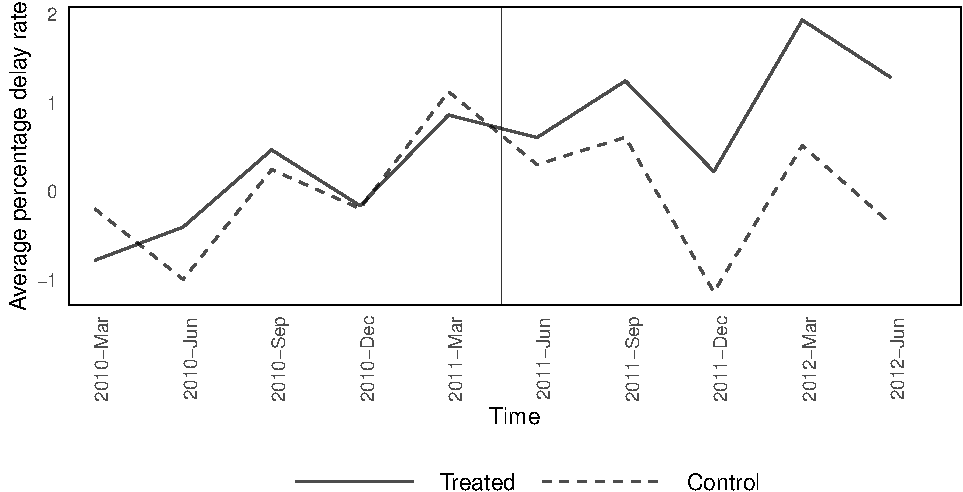
\includegraphics{qp_first_pc_delay_clean_control_time_independent_files/figure-latex/demeaned_plot_one_type-1.pdf}

\hypertarget{baseline-regressions}{%
\section{Baseline Regressions}\label{baseline-regressions}}

\[ PercentDelay_{it} = \beta_0 + \beta_1 Treat_i + \beta_2 Post_t + \beta_3 (Treat_i \times Post_t) + e_{it}\]

\[ \begin{aligned} PercentDelay_{it} &=& \alpha+\beta_0 Treat_i + \beta_1 Post_t + \beta_2 (Treat_i \times Post_t)\\
&+&  X_i + (Post_t \times X_i) + \mu_t + \theta_{firm} + \lambda_{task}+ \epsilon_{it}
\end{aligned}\]

\begin{table}[H] \centering 
  \caption{Effect of QuickPay on project delay rates} 
  \label{} 
\small 
\begin{tabular}{@{\extracolsep{-2pt}}lccccc} 
\\[-1.8ex]\hline 
\hline \\[-1.8ex] 
\\[-1.8ex] & \multicolumn{5}{c}{$PercentDelay_{it}$} \\ 
\\[-1.8ex] & (1) & (2) & (3) & (4) & (5)\\ 
\hline \\[-1.8ex] 
 $Treat_i$ & $-$1.76$^{***}$ & $-$1.36$^{***}$ & $-$1.41$^{***}$ & $-$0.92$^{***}$ & $-$0.93$^{***}$ \\ 
  & (0.11) & (0.11) & (0.11) & (0.11) & (0.11) \\ 
  & & & & & \\ 
 $Post_t$ & $-$0.21$^{*}$ & $-$5.58$^{***}$ &  &  &  \\ 
  & (0.12) & (0.78) &  &  &  \\ 
  & & & & & \\ 
 $Treat_i \times Post_t$ & 1.10$^{***}$ & 1.05$^{***}$ & 1.09$^{***}$ & 1.03$^{***}$ & 1.05$^{***}$ \\ 
  & (0.14) & (0.13) & (0.13) & (0.13) & (0.13) \\ 
  & & & & & \\ 
 Constant & 5.27$^{***}$ & 42.69$^{***}$ &  &  &  \\ 
  & (0.10) & (0.61) &  &  &  \\ 
  & & & & & \\ 
\hline \\[-1.8ex] 
Duration, Budget, Bids & No & Yes & Yes & Yes & Yes \\ 
$Post_t \times$  (Duration, Budget, Bids) & No & Yes & Yes & Yes & Yes \\ 
Project stage & No & Yes & Yes & Yes & Yes \\ 
Time fixed effects & No & No & Yes & Yes & Yes \\ 
Task fixed effects & No & No & No & Yes & Yes \\ 
Industry fixed effects & No & No & No & No & Yes \\ 
Observations & 223,244 & 201,738 & 201,738 & 201,738 & 201,738 \\ 
R$^{2}$ & 0.002 & 0.17 & 0.18 & 0.21 & 0.21 \\ 
Adjusted R$^{2}$ & 0.002 & 0.17 & 0.18 & 0.21 & 0.21 \\ 
\hline 
\hline \\[-1.8ex] 
\textit{Note:}  & \multicolumn{5}{r}{$^{*}$p$<$0.1; $^{**}$p$<$0.05; $^{***}$p$<$0.01} \\ 
 & \multicolumn{5}{r}{Each observation is a project-quarter.} \\ 
 & \multicolumn{5}{r}{SEs are robust and clustered at the project level.} \\ 
\end{tabular} 
\end{table}

\hypertarget{days-of-delay}{%
\subsection{Days of delay}\label{days-of-delay}}

\begin{table}[H] \centering 
  \caption{Effect of QuickPay on project delay rates} 
  \label{} 
\small 
\begin{tabular}{@{\extracolsep{-2pt}}lccccc} 
\\[-1.8ex]\hline 
\hline \\[-1.8ex] 
\\[-1.8ex] & \multicolumn{5}{c}{$DelayDays_{it}$} \\ 
\\[-1.8ex] & (1) & (2) & (3) & (4) & (5)\\ 
\hline \\[-1.8ex] 
 $Treat_i$ & $-$3.69$^{***}$ & $-$2.53$^{***}$ & $-$2.63$^{***}$ & $-$2.01$^{***}$ & $-$2.03$^{***}$ \\ 
  & (0.20) & (0.19) & (0.19) & (0.20) & (0.20) \\ 
  & & & & & \\ 
 $Post_t$ & 1.37$^{***}$ & $-$5.81$^{***}$ &  &  &  \\ 
  & (0.22) & (1.32) &  &  &  \\ 
  & & & & & \\ 
 $Treat_i \times Post_t$ & 1.65$^{***}$ & 2.03$^{***}$ & 2.13$^{***}$ & 2.00$^{***}$ & 2.02$^{***}$ \\ 
  & (0.26) & (0.26) & (0.26) & (0.25) & (0.26) \\ 
  & & & & & \\ 
 Constant & 9.36$^{***}$ & 55.41$^{***}$ &  &  &  \\ 
  & (0.17) & (0.98) &  &  &  \\ 
  & & & & & \\ 
\hline \\[-1.8ex] 
Duration, Budget, Bids & No & Yes & Yes & Yes & Yes \\ 
$Post_t \times$  (Duration, Budget, Bids) & No & Yes & Yes & Yes & Yes \\ 
Project stage & No & Yes & Yes & Yes & Yes \\ 
Time fixed effects & No & No & Yes & Yes & Yes \\ 
Task fixed effects & No & No & No & Yes & Yes \\ 
Industry fixed effects & No & No & No & No & Yes \\ 
Observations & 223,373 & 201,867 & 201,867 & 201,867 & 201,867 \\ 
R$^{2}$ & 0.004 & 0.14 & 0.14 & 0.17 & 0.17 \\ 
Adjusted R$^{2}$ & 0.004 & 0.14 & 0.14 & 0.17 & 0.17 \\ 
\hline 
\hline \\[-1.8ex] 
\textit{Note:}  & \multicolumn{5}{r}{$^{*}$p$<$0.1; $^{**}$p$<$0.05; $^{***}$p$<$0.01} \\ 
 & \multicolumn{5}{r}{Each observation is a project-quarter.} \\ 
 & \multicolumn{5}{r}{SEs are robust and clustered at the project level.} \\ 
\end{tabular} 
\end{table}

\hypertarget{event-study}{%
\section{Event study}\label{event-study}}

\(PercentDelay_{it}=\beta_0 + \beta_1 Treat_i + \beta_2 Treat_i \times Quarter_t + Controls + \gamma_{task} + \theta_{naics}+\lambda_{quarter}+\epsilon_{it}\)

\begin{verbatim}
## NOTE: 231,007 observations removed because of NA values (LHS: 209,501, RHS: 230,878).
\end{verbatim}

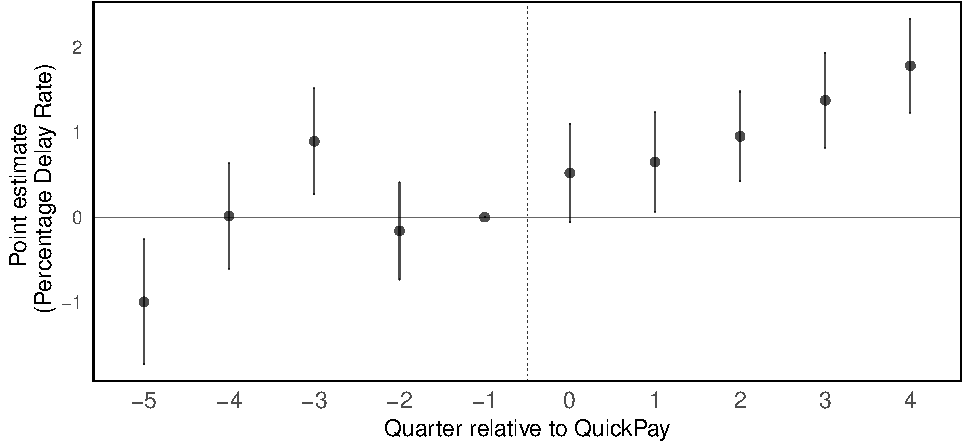
\includegraphics{qp_first_pc_delay_clean_control_time_independent_files/figure-latex/event_study-1.pdf}

\hypertarget{parallel-trends-test}{%
\section{Parallel Trends Test}\label{parallel-trends-test}}

\begin{table}[H] \centering 
  \caption{Linear Time Trend Before QuickPay} 
  \label{} 
\small 
\begin{tabular}{@{\extracolsep{-2pt}}lccccc} 
\\[-1.8ex]\hline 
\hline \\[-1.8ex] 
\\[-1.8ex] & \multicolumn{5}{c}{$PercentDelay_{it}$} \\ 
\\[-1.8ex] & (1) & (2) & (3) & (4) & (5)\\ 
\hline \\[-1.8ex] 
 $Treat_i$ & $-$1.37$^{***}$ & $-$0.90$^{**}$ & $-$0.91$^{**}$ & $-$0.44 & $-$0.51 \\ 
  & (0.41) & (0.40) & (0.40) & (0.41) & (0.41) \\ 
  & & & & & \\ 
 $QuarterNum$ & 0.42$^{***}$ & $-$1.22$^{**}$ &  &  &  \\ 
  & (0.08) & (0.49) &  &  &  \\ 
  & & & & & \\ 
 $Treat_i \times QuarterNum$ & $-$0.09 & $-$0.12 & $-$0.12 & $-$0.03 & $-$0.02 \\ 
  & (0.09) & (0.09) & (0.09) & (0.09) & (0.09) \\ 
  & & & & & \\ 
 Constant & 3.36$^{***}$ & 48.53$^{***}$ &  &  &  \\ 
  & (0.35) & (2.30) &  &  &  \\ 
  & & & & & \\ 
\hline \\[-1.8ex] 
Duration, Budget, Bids & No & Yes & Yes & Yes & Yes \\ 
$Post_t \times$  (Duration, Budget, Bids) & No & Yes & Yes & Yes & Yes \\ 
Project stage & No & Yes & Yes & Yes & Yes \\ 
Time fixed effects & No & No & Yes & Yes & Yes \\ 
Task fixed effects & No & No & No & Yes & Yes \\ 
Industry fixed effects & No & No & No & No & Yes \\ 
Observations & 84,367 & 77,984 & 77,984 & 77,984 & 77,984 \\ 
R$^{2}$ & 0.005 & 0.20 & 0.20 & 0.26 & 0.27 \\ 
Adjusted R$^{2}$ & 0.005 & 0.20 & 0.20 & 0.25 & 0.26 \\ 
\hline 
\hline \\[-1.8ex] 
\textit{Note:}  & \multicolumn{5}{r}{$^{*}$p$<$0.1; $^{**}$p$<$0.05; $^{***}$p$<$0.01} \\ 
 & \multicolumn{5}{r}{Each observation is a project-quarter.} \\ 
 & \multicolumn{5}{r}{SEs are robust and clustered at the project level.} \\ 
 & \multicolumn{5}{r}{Observations are for quarters before quickpay.} \\ 
\end{tabular} 
\end{table}

\hypertarget{placebo-test}{%
\section{Placebo Test}\label{placebo-test}}

{[}1{]} 3

\begin{table}[H] \centering 
  \caption{Placebo test: Treatment Time 2010-06-30} 
  \label{} 
\small 
\begin{tabular}{@{\extracolsep{-2pt}}lccccc} 
\\[-1.8ex]\hline 
\hline \\[-1.8ex] 
\\[-1.8ex] & \multicolumn{5}{c}{$PercentDelay_{it}$} \\ 
\\[-1.8ex] & (1) & (2) & (3) & (4) & (5)\\ 
\hline \\[-1.8ex] 
 $Treat_i$ & $-$4.19$^{***}$ & $-$4.98$^{***}$ & $-$5.00$^{***}$ & $-$2.59$^{***}$ & $-$2.71$^{***}$ \\ 
  & (0.71) & (0.73) & (0.73) & (0.71) & (0.71) \\ 
  & & & & & \\ 
 $Post$ & 0.22 & $-$13.48$^{***}$ &  &  &  \\ 
  & (0.65) & (4.65) &  &  &  \\ 
  & & & & & \\ 
 $Treat_i \times Post$ & 1.10 & 2.09$^{***}$ & 2.04$^{***}$ & 1.39$^{*}$ & 1.47$^{**}$ \\ 
  & (0.74) & (0.76) & (0.76) & (0.74) & (0.74) \\ 
  & & & & & \\ 
 Constant & 8.99$^{***}$ & 96.80$^{***}$ &  &  &  \\ 
  & (0.63) & (4.39) &  &  &  \\ 
  & & & & & \\ 
\hline \\[-1.8ex] 
Duration, Budget, Bids & No & Yes & Yes & Yes & Yes \\ 
$Post_t \times$  (Duration, Budget, Bids) & No & Yes & Yes & Yes & Yes \\ 
Project stage & No & Yes & Yes & Yes & Yes \\ 
Time fixed effects & No & No & Yes & Yes & Yes \\ 
Task fixed effects & No & No & No & Yes & Yes \\ 
Industry fixed effects & No & No & No & No & Yes \\ 
Observations & 84,367 & 77,984 & 77,984 & 77,984 & 77,984 \\ 
R$^{2}$ & 0.003 & 0.20 & 0.21 & 0.26 & 0.27 \\ 
Adjusted R$^{2}$ & 0.003 & 0.20 & 0.21 & 0.25 & 0.26 \\ 
\hline 
\hline \\[-1.8ex] 
\textit{Note:}  & \multicolumn{5}{r}{$^{*}$p$<$0.1; $^{**}$p$<$0.05; $^{***}$p$<$0.01} \\ 
 & \multicolumn{5}{r}{Each observation is a project-quarter.} \\ 
 & \multicolumn{5}{r}{SEs are robust and clustered at the project level.} \\ 
 & \multicolumn{5}{r}{Observations are for quarters before quickpay.} \\ 
\end{tabular} 
\end{table}

{[}1{]} 4

\begin{table}[H] \centering 
  \caption{Placebo test: Treatment Time 2010-09-30} 
  \label{} 
\small 
\begin{tabular}{@{\extracolsep{-2pt}}lccccc} 
\\[-1.8ex]\hline 
\hline \\[-1.8ex] 
\\[-1.8ex] & \multicolumn{5}{c}{$PercentDelay_{it}$} \\ 
\\[-1.8ex] & (1) & (2) & (3) & (4) & (5)\\ 
\hline \\[-1.8ex] 
 $Treat_i$ & $-$2.85$^{***}$ & $-$3.46$^{***}$ & $-$3.47$^{***}$ & $-$1.64$^{***}$ & $-$1.73$^{***}$ \\ 
  & (0.42) & (0.42) & (0.42) & (0.42) & (0.42) \\ 
  & & & & & \\ 
 $Post$ & 1.66$^{***}$ & $-$10.63$^{***}$ &  &  &  \\ 
  & (0.41) & (3.10) &  &  &  \\ 
  & & & & & \\ 
 $Treat_i \times Post$ & $-$0.45 & 0.44 & 0.43 & 0.41 & 0.47 \\ 
  & (0.48) & (0.48) & (0.48) & (0.48) & (0.48) \\ 
  & & & & & \\ 
 Constant & 7.93$^{***}$ & 92.99$^{***}$ &  &  &  \\ 
  & (0.36) & (2.69) &  &  &  \\ 
  & & & & & \\ 
\hline \\[-1.8ex] 
Duration, Budget, Bids & No & Yes & Yes & Yes & Yes \\ 
$Post_t \times$  (Duration, Budget, Bids) & No & Yes & Yes & Yes & Yes \\ 
Project stage & No & Yes & Yes & Yes & Yes \\ 
Time fixed effects & No & No & Yes & Yes & Yes \\ 
Task fixed effects & No & No & No & Yes & Yes \\ 
Industry fixed effects & No & No & No & No & Yes \\ 
Observations & 84,367 & 77,984 & 77,984 & 77,984 & 77,984 \\ 
R$^{2}$ & 0.004 & 0.21 & 0.21 & 0.26 & 0.27 \\ 
Adjusted R$^{2}$ & 0.004 & 0.20 & 0.21 & 0.25 & 0.26 \\ 
\hline 
\hline \\[-1.8ex] 
\textit{Note:}  & \multicolumn{5}{r}{$^{*}$p$<$0.1; $^{**}$p$<$0.05; $^{***}$p$<$0.01} \\ 
 & \multicolumn{5}{r}{Each observation is a project-quarter.} \\ 
 & \multicolumn{5}{r}{SEs are robust and clustered at the project level.} \\ 
 & \multicolumn{5}{r}{Observations are for quarters before quickpay.} \\ 
\end{tabular} 
\end{table}

{[}1{]} 5

\begin{table}[H] \centering 
  \caption{Placebo test: Treatment Time 2010-12-31} 
  \label{} 
\small 
\begin{tabular}{@{\extracolsep{-2pt}}lccccc} 
\\[-1.8ex]\hline 
\hline \\[-1.8ex] 
\\[-1.8ex] & \multicolumn{5}{c}{$PercentDelay_{it}$} \\ 
\\[-1.8ex] & (1) & (2) & (3) & (4) & (5)\\ 
\hline \\[-1.8ex] 
 $Treat_i$ & $-$2.86$^{***}$ & $-$2.40$^{***}$ & $-$2.42$^{***}$ & $-$0.75$^{**}$ & $-$0.82$^{**}$ \\ 
  & (0.32) & (0.32) & (0.32) & (0.34) & (0.34) \\ 
  & & & & & \\ 
 $Post$ & 0.99$^{***}$ & $-$15.11$^{***}$ &  &  &  \\ 
  & (0.37) & (2.65) &  &  &  \\ 
  & & & & & \\ 
 $Treat_i \times Post$ & $-$0.60 & $-$1.32$^{***}$ & $-$1.27$^{***}$ & $-$0.93$^{**}$ & $-$0.89$^{**}$ \\ 
  & (0.43) & (0.43) & (0.43) & (0.45) & (0.45) \\ 
  & & & & & \\ 
 Constant & 8.65$^{***}$ & 93.54$^{***}$ &  &  &  \\ 
  & (0.28) & (2.03) &  &  &  \\ 
  & & & & & \\ 
\hline \\[-1.8ex] 
Duration, Budget, Bids & No & Yes & Yes & Yes & Yes \\ 
$Post_t \times$  (Duration, Budget, Bids) & No & Yes & Yes & Yes & Yes \\ 
Project stage & No & Yes & Yes & Yes & Yes \\ 
Time fixed effects & No & No & Yes & Yes & Yes \\ 
Task fixed effects & No & No & No & Yes & Yes \\ 
Industry fixed effects & No & No & No & No & Yes \\ 
Observations & 84,367 & 77,984 & 77,984 & 77,984 & 77,984 \\ 
R$^{2}$ & 0.003 & 0.21 & 0.21 & 0.26 & 0.27 \\ 
Adjusted R$^{2}$ & 0.003 & 0.21 & 0.21 & 0.25 & 0.26 \\ 
\hline 
\hline \\[-1.8ex] 
\textit{Note:}  & \multicolumn{5}{r}{$^{*}$p$<$0.1; $^{**}$p$<$0.05; $^{***}$p$<$0.01} \\ 
 & \multicolumn{5}{r}{Each observation is a project-quarter.} \\ 
 & \multicolumn{5}{r}{SEs are robust and clustered at the project level.} \\ 
 & \multicolumn{5}{r}{Observations are for quarters before quickpay.} \\ 
\end{tabular} 
\end{table}

\hypertarget{summary-statistics-full-sample}{%
\section{Summary statistics {[}Full
sample{]}}\label{summary-statistics-full-sample}}

\hypertarget{congestion-effect}{%
\section{Congestion Effect}\label{congestion-effect}}

\hypertarget{number-of-projects-per-contractor}{%
\subsection{Number of projects per
contractor}\label{number-of-projects-per-contractor}}

\hypertarget{contractors-holding-only-small-or-only-large-projects}{%
\subsubsection{Contractors holding only small or only large
projects}\label{contractors-holding-only-small-or-only-large-projects}}

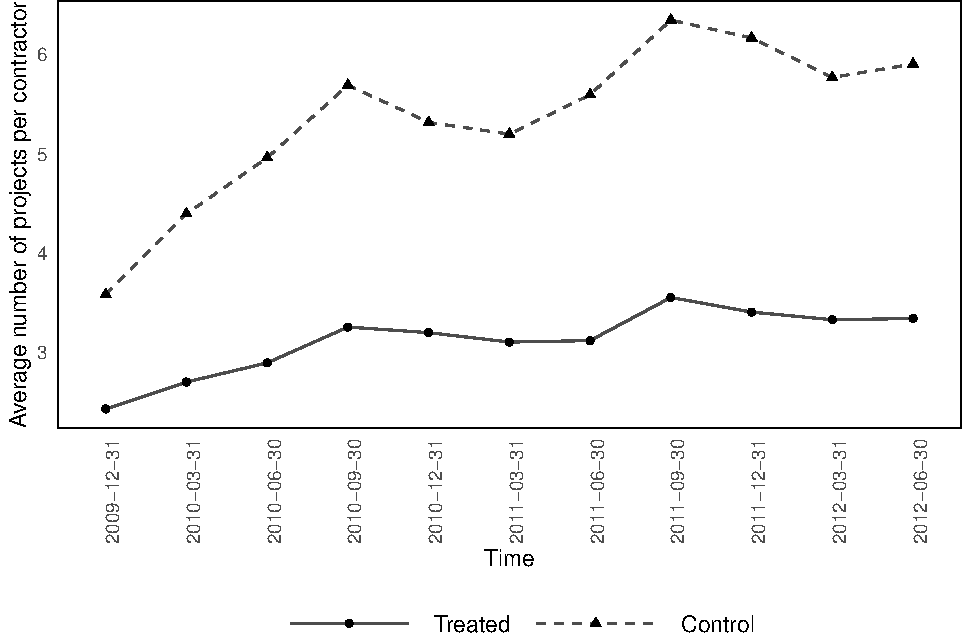
\includegraphics{qp_first_pc_delay_clean_control_time_independent_files/figure-latex/num_projects_0-1.pdf}

\begin{table}[H] \centering 
  \caption{Num Contractor Projects and QuickPay reform} 
  \label{} 
\small 
\begin{tabular}{@{\extracolsep{-2pt}}lcc} 
\\[-1.8ex]\hline 
\hline \\[-1.8ex] 
\\[-1.8ex] & \multicolumn{2}{c}{Number of projects} \\ 
\\[-1.8ex] & (1) & (2)\\ 
\hline \\[-1.8ex] 
 $Treat_i$ & $-$2.03$^{***}$ & $-$2.03$^{***}$ \\ 
  & (0.39) & (0.39) \\ 
  & & \\ 
 $Post_t$ & 0.94$^{**}$ &  \\ 
  & (0.41) &  \\ 
  & & \\ 
 $Treat_i \times Post_t$ & $-$0.58 & $-$0.58 \\ 
  & (0.41) & (0.41) \\ 
  & & \\ 
 Constant & 5.03$^{***}$ &  \\ 
  & (0.38) &  \\ 
  & & \\ 
\hline \\[-1.8ex] 
Time fixed effects & No & Yes \\ 
Observations & 84,391 & 84,391 \\ 
R$^{2}$ & 0.005 & 0.01 \\ 
Adjusted R$^{2}$ & 0.005 & 0.01 \\ 
\hline 
\hline \\[-1.8ex] 
\textit{Note:}  & \multicolumn{2}{r}{$^{*}$p$<$0.1; $^{**}$p$<$0.05; $^{***}$p$<$0.01} \\ 
 & \multicolumn{2}{r}{Each observation is a contractor-quarter.} \\ 
 & \multicolumn{2}{r}{SEs are robust and clustered at the contractor level.} \\ 
 & \multicolumn{2}{r}{Sample restricted to contractors performing only one type of project.} \\ 
\end{tabular} 
\end{table}

\hypertarget{contractors-holding-at-least-one-small-project-are-treated}{%
\subsubsection{Contractors holding at least one small project are
``treated''}\label{contractors-holding-at-least-one-small-project-are-treated}}

\hypertarget{total-budget}{%
\subsection{Total budget}\label{total-budget}}

\hypertarget{contractors-holding-only-small-or-only-large-projects-1}{%
\subsubsection{Contractors holding only small or only large
projects}\label{contractors-holding-only-small-or-only-large-projects-1}}

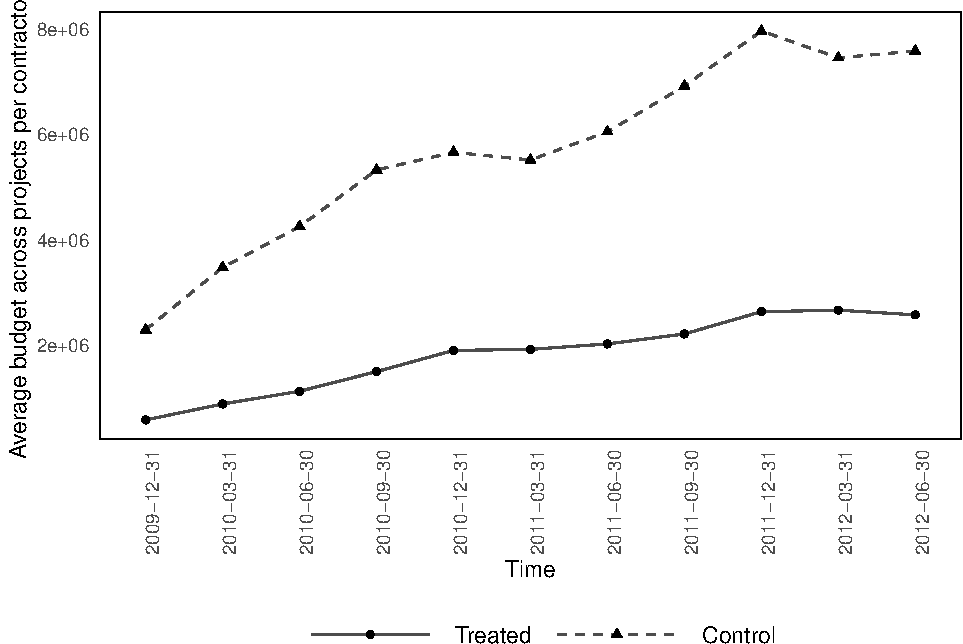
\includegraphics{qp_first_pc_delay_clean_control_time_independent_files/figure-latex/budget_0-1.pdf}

\begin{table}[H] \centering 
  \caption{Contractor Project Budget and QuickPay reform} 
  \label{} 
\small 
\begin{tabular}{@{\extracolsep{-2pt}}lcc} 
\\[-1.8ex]\hline 
\hline \\[-1.8ex] 
\\[-1.8ex] & \multicolumn{2}{c}{Total budget} \\ 
\\[-1.8ex] & (1) & (2)\\ 
\hline \\[-1.8ex] 
 $Treat_i$ & $-$2,503,033.00$^{***}$ & $-$2,497,737.00$^{***}$ \\ 
  & (454,885.70) & (456,972.80) \\ 
  & & \\ 
 $Post_t$ & 1,715,503.00$^{***}$ &  \\ 
  & (229,333.50) &  \\ 
  & & \\ 
 $Treat_i \times Post_t$ & $-$953,041.30$^{***}$ & $-$955,237.70$^{***}$ \\ 
  & (231,908.60) & (233,131.80) \\ 
  & & \\ 
 Constant & 3,666,740.00$^{***}$ &  \\ 
  & (453,287.80) &  \\ 
  & & \\ 
\hline \\[-1.8ex] 
Time fixed effects & No & Yes \\ 
Observations & 84,391 & 84,391 \\ 
R$^{2}$ & 0.01 & 0.02 \\ 
Adjusted R$^{2}$ & 0.01 & 0.01 \\ 
\hline 
\hline \\[-1.8ex] 
\textit{Note:}  & \multicolumn{2}{r}{$^{*}$p$<$0.1; $^{**}$p$<$0.05; $^{***}$p$<$0.01} \\ 
 & \multicolumn{2}{r}{Each observation is a contractor-quarter.} \\ 
 & \multicolumn{2}{r}{SEs are robust and clustered at the contractor level.} \\ 
 & \multicolumn{2}{r}{Sample restricted to contractors performing only one type of project.} \\ 
\end{tabular} 
\end{table}

\hypertarget{number-of-tasks}{%
\subsection{Number of tasks}\label{number-of-tasks}}

\hypertarget{contractors-holding-only-small-or-only-large-projects-2}{%
\subsubsection{Contractors holding only small or only large
projects}\label{contractors-holding-only-small-or-only-large-projects-2}}

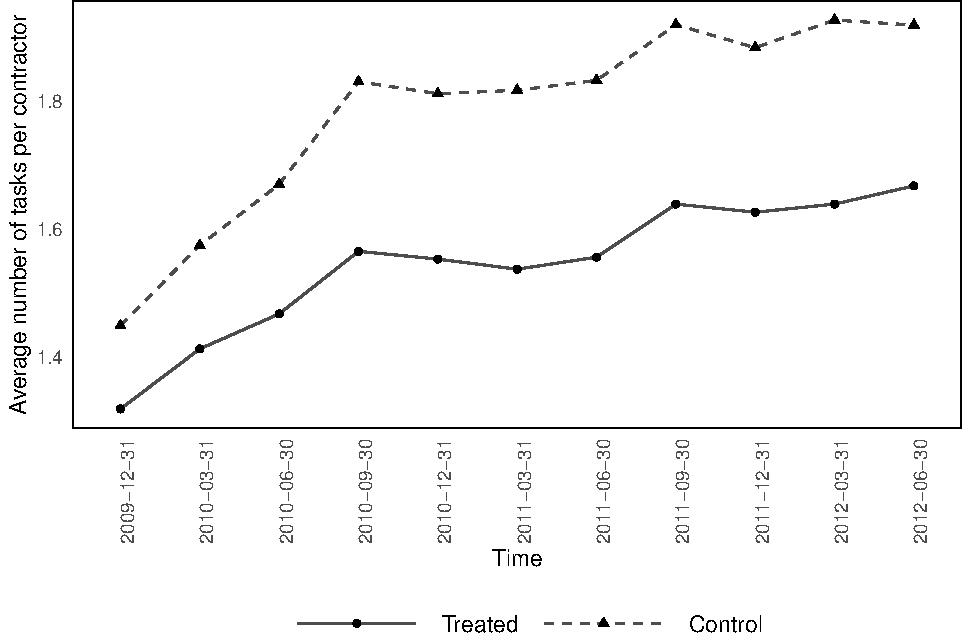
\includegraphics{qp_first_pc_delay_clean_control_time_independent_files/figure-latex/tasks_0-1.pdf}

\begin{table}[H] \centering 
  \caption{Contractor Project Tasks and QuickPay reform} 
  \label{} 
\small 
\begin{tabular}{@{\extracolsep{-2pt}}lcc} 
\\[-1.8ex]\hline 
\hline \\[-1.8ex] 
\\[-1.8ex] & \multicolumn{2}{c}{Number of tasks} \\ 
\\[-1.8ex] & (1) & (2)\\ 
\hline \\[-1.8ex] 
 $Treat_i$ & $-$0.23$^{***}$ & $-$0.23$^{***}$ \\ 
  & (0.04) & (0.04) \\ 
  & & \\ 
 $Post_t$ & 0.17$^{***}$ &  \\ 
  & (0.02) &  \\ 
  & & \\ 
 $Treat_i \times Post_t$ & $-$0.04 & $-$0.04 \\ 
  & (0.03) & (0.03) \\ 
  & & \\ 
 Constant & 1.73$^{***}$ &  \\ 
  & (0.04) &  \\ 
  & & \\ 
\hline \\[-1.8ex] 
Time fixed effects & No & Yes \\ 
Observations & 84,391 & 84,391 \\ 
R$^{2}$ & 0.01 & 0.01 \\ 
Adjusted R$^{2}$ & 0.01 & 0.01 \\ 
\hline 
\hline \\[-1.8ex] 
\textit{Note:}  & \multicolumn{2}{r}{$^{*}$p$<$0.1; $^{**}$p$<$0.05; $^{***}$p$<$0.01} \\ 
 & \multicolumn{2}{r}{Each observation is a contractor-quarter.} \\ 
 & \multicolumn{2}{r}{SEs are robust and clustered at the contractor level.} \\ 
 & \multicolumn{2}{r}{Sample restricted to contractors performing only one type of project.} \\ 
\end{tabular} 
\end{table}

\hypertarget{project-portfolio-spillover-effect}{%
\section{Project portfolio: Spillover
effect}\label{project-portfolio-spillover-effect}}

\hypertarget{regression-1-did-on-large-projects}{%
\subsection{Regression 1: DID on large
projects}\label{regression-1-did-on-large-projects}}

\begin{itemize}
\tightlist
\item
  Sample restricted to large projects only.
\item
  Treat is an indicator that equals one for LARGE projects that have at
  least one parallel small project in the same quarter, and is zero
  otherwise.
\end{itemize}

\begin{table}[H] \centering 
  \caption{Project Portfolio and QuickPay reform} 
  \label{} 
\small 
\begin{tabular}{@{\extracolsep{-10pt}}lccccc} 
\\[-1.8ex]\hline 
\hline \\[-1.8ex] 
\\[-1.8ex] & \multicolumn{5}{c}{$PercentDelay_{it}$} \\ 
\\[-1.8ex] & (1) & (2) & (3) & (4) & (5)\\ 
\hline \\[-1.8ex] 
 $Treat_i$ & 4.41$^{***}$ & 0.70$^{***}$ & 0.64$^{***}$ & 1.15$^{***}$ & 1.16$^{***}$ \\ 
  & (0.31) & (0.20) & (0.20) & (0.20) & (0.20) \\ 
  & & & & & \\ 
 $Post_t$ & $-$0.10 & $-$13.38$^{***}$ &  &  &  \\ 
  & (0.12) & (1.17) &  &  &  \\ 
  & & & & & \\ 
 $Treat_i \times Post_t$ & $-$1.17$^{***}$ & 0.02 & 0.03 & $-$0.65$^{**}$ & $-$0.56$^{**}$ \\ 
  & (0.36) & (0.26) & (0.26) & (0.26) & (0.26) \\ 
  & & & & & \\ 
 Constant & 5.59$^{***}$ & 63.76$^{***}$ &  &  &  \\ 
  & (0.10) & (0.89) &  &  &  \\ 
  & & & & & \\ 
\hline \\[-1.8ex] 
Duration, Budget, Bids & No & Yes & Yes & Yes & Yes \\ 
$Post_t \times $  (Duration, Budget, Bids) & No & Yes & Yes & Yes & Yes \\ 
Project stage & No & Yes & Yes & Yes & Yes \\ 
Time fixed effects & No & No & Yes & Yes & Yes \\ 
Task fixed effects & No & No & No & Yes & Yes \\ 
Industry fixed effects & No & No & No & No & Yes \\ 
Observations & 117,787 & 110,601 & 110,601 & 110,601 & 110,601 \\ 
R$^{2}$ & 0.01 & 0.26 & 0.26 & 0.30 & 0.30 \\ 
Adjusted R$^{2}$ & 0.01 & 0.26 & 0.26 & 0.29 & 0.29 \\ 
\hline 
\hline \\[-1.8ex] 
\textit{Note:}  & \multicolumn{5}{r}{$^{*}$p$<$0.1; $^{**}$p$<$0.05; $^{***}$p$<$0.01} \\ 
 & \multicolumn{5}{r}{Each observation is a project-quarter.} \\ 
 & \multicolumn{5}{r}{SEs are robust and clustered at the project level.} \\ 
 & \multicolumn{5}{r}{Sample restricted to large projects only.} \\ 
\end{tabular} 
\end{table}

\hypertarget{regression-2-incremental-effect-on-small-project-with-existing-large-project}{%
\subsection{Regression 2: Incremental effect on small project with
existing large
project}\label{regression-2-incremental-effect-on-small-project-with-existing-large-project}}

\begin{itemize}
\tightlist
\item
  \(Treat_{i,l}\) is an indicator that equals 1 for small projects with
  co-existing large projects in a given quarter, and is zero otherwise.

  \begin{itemize}
  \tightlist
  \item
    This depends on time, though we are not defining it explicitly.
  \end{itemize}
\item
  \(Treat_{i,l}=1 \implies Treat_i = 1\). This means we have:

  \begin{itemize}
  \tightlist
  \item
    \(Treat_{i,l} \times Post_t = Treat_i \times Treat_{i,l} \times Post_t\)
  \item
    \(Treat_{i,l} \times Treat_i = Treat_{i,l}\)
  \end{itemize}
\item
  Large projects with parallel small projects are removed to get a clean
  control group.
\end{itemize}

\begin{table}[H] \centering 
  \caption{(Incremental effect) Project Portfolio and QuickPay reform} 
  \label{} 
\small 
\begin{tabular}{@{\extracolsep{-2pt}}lccccc} 
\\[-1.8ex]\hline 
\hline \\[-1.8ex] 
\\[-1.8ex] & \multicolumn{5}{c}{$PercentDelay_{it}$  } \\ 
\\[-1.8ex] & (1) & (2) & (3) & (4) & (5)\\ 
\hline \\[-1.8ex] 
 $Treat_i$ & $-$1.38$^{***}$ & $-$1.15$^{***}$ & $-$1.19$^{***}$ & $-$0.85$^{***}$ & $-$0.87$^{***}$ \\ 
  & (0.12) & (0.11) & (0.11) & (0.11) & (0.11) \\ 
  & & & & & \\ 
 $Treat_{i,l}$ & $-$2.16$^{***}$ & $-$1.28$^{***}$ & $-$1.30$^{***}$ & $-$0.38$^{***}$ & $-$0.34$^{***}$ \\ 
  & (0.12) & (0.12) & (0.12) & (0.11) & (0.11) \\ 
  & & & & & \\ 
 $Post_t$ & $-$0.21$^{*}$ & $-$5.55$^{***}$ &  &  &  \\ 
  & (0.12) & (0.78) &  &  &  \\ 
  & & & & & \\ 
 $Treat_i \times Post_t$ & 1.25$^{***}$ & 1.19$^{***}$ & 1.23$^{***}$ & 1.15$^{***}$ & 1.16$^{***}$ \\ 
  & (0.14) & (0.14) & (0.14) & (0.14) & (0.14) \\ 
  & & & & & \\ 
 $Treat_{i,l} \times Post_t$ & $-$0.63$^{***}$ & $-$0.62$^{***}$ & $-$0.62$^{***}$ & $-$0.61$^{***}$ & $-$0.56$^{***}$ \\ 
  & (0.15) & (0.15) & (0.15) & (0.15) & (0.15) \\ 
  & & & & & \\ 
 Constant & 5.27$^{***}$ & 42.71$^{***}$ &  &  &  \\ 
  & (0.10) & (0.60) &  &  &  \\ 
  & & & & & \\ 
\hline \\[-1.8ex] 
Duration, Budget, Bids & No & Yes & Yes & Yes & Yes \\ 
$Post_t \times $  (Duration, Budget, Bids) & No & Yes & Yes & Yes & Yes \\ 
Project stage & No & Yes & Yes & Yes & Yes \\ 
Time fixed effects & No & No & Yes & Yes & Yes \\ 
Task fixed effects & No & No & No & Yes & Yes \\ 
Industry fixed effects & No & No & No & No & Yes \\ 
Observations & 223,244 & 201,738 & 201,738 & 201,738 & 201,738 \\ 
R$^{2}$ & 0.005 & 0.18 & 0.18 & 0.21 & 0.21 \\ 
Adjusted R$^{2}$ & 0.005 & 0.18 & 0.18 & 0.21 & 0.21 \\ 
\hline 
\hline \\[-1.8ex] 
\textit{Note:}  & \multicolumn{5}{r}{$^{*}$p$<$0.1; $^{**}$p$<$0.05; $^{***}$p$<$0.01} \\ 
 & \multicolumn{5}{r}{Each observation is a project-quarter.} \\ 
 & \multicolumn{5}{r}{SEs are robust and clustered at the project level.} \\ 
 & \multicolumn{5}{r}{Large projects with parallel small projects are removed.} \\ 
\end{tabular} 
\end{table}

\hypertarget{regression-3-total-effect-on-small-project-with-existing-large-project}{%
\subsection{Regression 3: Total effect on small project with existing
large
project}\label{regression-3-total-effect-on-small-project-with-existing-large-project}}

\begin{itemize}
\tightlist
\item
  \(Treat_{i,l}\) is an indicator that equals 1 for small projects with
  co-existing large projects, and is zero otherwise.
\item
  \(Treat_{i,s}\) is an indicator that equals 1 for small projects
  without co-existing large projects, and is zero otherwise.
\item
  Large projects with parallel small projects are removed to get a clean
  control group.
\end{itemize}

\begin{table}[H] \centering 
  \caption{(Total effect) Project Portfolio and QuickPay reform} 
  \label{} 
\small 
\begin{tabular}{@{\extracolsep{-2pt}}lccccc} 
\\[-1.8ex]\hline 
\hline \\[-1.8ex] 
\\[-1.8ex] & \multicolumn{5}{c}{$PercentDelay_{it}$  } \\ 
\\[-1.8ex] & (1) & (2) & (3) & (4) & (5)\\ 
\hline \\[-1.8ex] 
 $Treat_{i,s}$ & $-$1.38$^{***}$ & $-$1.15$^{***}$ & $-$1.19$^{***}$ & $-$0.85$^{***}$ & $-$0.87$^{***}$ \\ 
  & (0.12) & (0.11) & (0.11) & (0.11) & (0.11) \\ 
  & & & & & \\ 
 $Treat_{i,l}$ & $-$3.54$^{***}$ & $-$2.42$^{***}$ & $-$2.49$^{***}$ & $-$1.24$^{***}$ & $-$1.21$^{***}$ \\ 
  & (0.14) & (0.14) & (0.14) & (0.13) & (0.14) \\ 
  & & & & & \\ 
 $Post_t$ & $-$0.21$^{*}$ & $-$5.55$^{***}$ &  &  &  \\ 
  & (0.12) & (0.78) &  &  &  \\ 
  & & & & & \\ 
 $Treat_{i,s} \times Post_t$ & 1.25$^{***}$ & 1.19$^{***}$ & 1.23$^{***}$ & 1.15$^{***}$ & 1.16$^{***}$ \\ 
  & (0.14) & (0.14) & (0.14) & (0.14) & (0.14) \\ 
  & & & & & \\ 
 $Treat_{i,l} \times Post_t$ & 0.62$^{***}$ & 0.58$^{***}$ & 0.62$^{***}$ & 0.53$^{***}$ & 0.60$^{***}$ \\ 
  & (0.17) & (0.17) & (0.17) & (0.17) & (0.17) \\ 
  & & & & & \\ 
 Constant & 5.27$^{***}$ & 42.71$^{***}$ &  &  &  \\ 
  & (0.10) & (0.60) &  &  &  \\ 
  & & & & & \\ 
\hline \\[-1.8ex] 
Duration, Budget, Bids & No & Yes & Yes & Yes & Yes \\ 
$Post_t \times $  (Duration, Budget, Bids) & No & Yes & Yes & Yes & Yes \\ 
Project stage & No & Yes & Yes & Yes & Yes \\ 
Time fixed effects & No & No & Yes & Yes & Yes \\ 
Task fixed effects & No & No & No & Yes & Yes \\ 
Industry fixed effects & No & No & No & No & Yes \\ 
Observations & 223,244 & 201,738 & 201,738 & 201,738 & 201,738 \\ 
R$^{2}$ & 0.005 & 0.18 & 0.18 & 0.21 & 0.21 \\ 
Adjusted R$^{2}$ & 0.005 & 0.18 & 0.18 & 0.21 & 0.21 \\ 
\hline 
\hline \\[-1.8ex] 
\textit{Note:}  & \multicolumn{5}{r}{$^{*}$p$<$0.1; $^{**}$p$<$0.05; $^{***}$p$<$0.01} \\ 
 & \multicolumn{5}{r}{Each observation is a project-quarter.} \\ 
 & \multicolumn{5}{r}{SEs are robust and clustered at the project level.} \\ 
 & \multicolumn{5}{r}{Large projects with parallel small projects are removed.} \\ 
\end{tabular} 
\end{table}

\hypertarget{project-stage}{%
\section{Project Stage}\label{project-stage}}

\begin{itemize}
\tightlist
\item
  \(t\) indicates the end of the quarter
\item
  We want to get stage of the project at the beginning of a given
  quarter (before any delays materialize)
\end{itemize}

\(Stage_{it}=\frac{ActionDate_{t-1}-StartDate_i}{Duration_{i,t-1}}\)
\(Stage_{it}=\frac{(t-1)-StartDate_i}{Duration_{i,t-1}}\)

\hypertarget{stage-quintile}{%
\subsection{Stage Quintile}\label{stage-quintile}}

\hypertarget{logged-stage-regressions}{%
\subsection{Logged Stage Regressions}\label{logged-stage-regressions}}

\begin{table}[H] \centering 
  \caption{Project Stage and QuickPay reform} 
  \label{} 
\small 
\begin{tabular}{@{\extracolsep{-2pt}}lccccc} 
\\[-1.8ex]\hline 
\hline \\[-1.8ex] 
\\[-1.8ex] & \multicolumn{5}{c}{$PercentDelay_{it}$  } \\ 
\\[-1.8ex] & (1) & (2) & (3) & (4) & (5)\\ 
\hline \\[-1.8ex] 
 $Treat_i$ & $-$2.65$^{***}$ & $-$1.71$^{***}$ & $-$1.79$^{***}$ & $-$1.35$^{***}$ & $-$1.38$^{***}$ \\ 
  & (0.23) & (0.21) & (0.21) & (0.20) & (0.20) \\ 
  & & & & & \\ 
 Log(Stage) & 3.16$^{***}$ & 2.51$^{***}$ & 2.46$^{***}$ & 2.53$^{***}$ & 2.53$^{***}$ \\ 
  & (0.08) & (0.07) & (0.07) & (0.07) & (0.07) \\ 
  & & & & & \\ 
 $Post_t$ & $-$1.33$^{***}$ & $-$5.06$^{***}$ &  &  &  \\ 
  & (0.23) & (0.80) &  &  &  \\ 
  & & & & & \\ 
 $Treat_i \times Post_t$ & 2.06$^{***}$ & 1.82$^{***}$ & 1.89$^{***}$ & 1.89$^{***}$ & 1.93$^{***}$ \\ 
  & (0.28) & (0.25) & (0.25) & (0.25) & (0.25) \\ 
  & & & & & \\ 
 $Treat_i \times$ Log(Stage) & $-$0.70$^{***}$ & $-$0.20$^{**}$ & $-$0.23$^{**}$ & $-$0.27$^{***}$ & $-$0.28$^{***}$ \\ 
  & (0.10) & (0.09) & (0.09) & (0.09) & (0.09) \\ 
  & & & & & \\ 
 $Post_t \times$ Log(Stage) & $-$0.06 & 0.47$^{***}$ & 0.49$^{***}$ & 0.23$^{**}$ & 0.22$^{**}$ \\ 
  & (0.10) & (0.09) & (0.09) & (0.09) & (0.09) \\ 
  & & & & & \\ 
 $Treat_i \times Post_t \times$ Log(Stage) & 0.59$^{***}$ & 0.54$^{***}$ & 0.56$^{***}$ & 0.61$^{***}$ & 0.62$^{***}$ \\ 
  & (0.12) & (0.11) & (0.11) & (0.11) & (0.11) \\ 
  & & & & & \\ 
 Constant & 10.20$^{***}$ & 42.59$^{***}$ &  &  &  \\ 
  & (0.19) & (0.62) &  &  &  \\ 
  & & & & & \\ 
\hline \\[-1.8ex] 
Duration, Budget, Bids & No & Yes & Yes & Yes & Yes \\ 
$Post_t \times $  (Duration, Budget, Bids) & No & Yes & Yes & Yes & Yes \\ 
Time fixed effects & No & No & Yes & Yes & Yes \\ 
Task fixed effects & No & No & No & Yes & Yes \\ 
Industry fixed effects & No & No & No & No & Yes \\ 
Observations & 223,213 & 201,738 & 201,738 & 201,738 & 201,738 \\ 
R$^{2}$ & 0.06 & 0.18 & 0.18 & 0.21 & 0.22 \\ 
Adjusted R$^{2}$ & 0.06 & 0.18 & 0.18 & 0.21 & 0.21 \\ 
\hline 
\hline \\[-1.8ex] 
\textit{Note:}  & \multicolumn{5}{r}{$^{*}$p$<$0.1; $^{**}$p$<$0.05; $^{***}$p$<$0.01} \\ 
 & \multicolumn{5}{r}{Each observation is a project-quarter.} \\ 
 & \multicolumn{5}{r}{SEs are robust and clustered at the project level.} \\ 
\end{tabular} 
\end{table}

\hypertarget{contract-financing-projects-active-onbefore-june-2010}{%
\section{Contract Financing (Projects active on/before June
2010)}\label{contract-financing-projects-active-onbefore-june-2010}}

\begin{itemize}
\tightlist
\item
  \(CF=1\) if project was receiving contract financing
\item
  Sample restricted to projects that started on or before June 2010
\item
  Jobs act was launched in Sept 2010
\end{itemize}

\begin{table}[H] \centering 
  \caption{Contract Financing and QuickPay reform} 
  \label{} 
\small 
\begin{tabular}{@{\extracolsep{-2pt}}lccccc} 
\\[-1.8ex]\hline 
\hline \\[-1.8ex] 
\\[-1.8ex] & \multicolumn{5}{c}{$PercentDelay_{it}$  } \\ 
\\[-1.8ex] & (1) & (2) & (3) & (4) & (5)\\ 
\hline \\[-1.8ex] 
 $Treat_i$ & $-$2.11$^{***}$ & $-$1.27$^{***}$ & $-$1.38$^{***}$ & $-$0.66$^{***}$ & $-$0.69$^{***}$ \\ 
  & (0.16) & (0.15) & (0.15) & (0.16) & (0.16) \\ 
  & & & & & \\ 
 $Post_t$ & 1.44$^{***}$ & $-$9.57$^{***}$ &  &  &  \\ 
  & (0.28) & (2.62) &  &  &  \\ 
  & & & & & \\ 
 $CF_i$ & 1.32$^{***}$ & 1.58$^{***}$ & 1.34$^{***}$ & $-$0.56$^{*}$ & $-$0.64$^{*}$ \\ 
  & (0.37) & (0.32) & (0.31) & (0.34) & (0.34) \\ 
  & & & & & \\ 
 $Treat_i \times Post_t$ & $-$0.03 & 2.42$^{***}$ & 2.52$^{***}$ & 2.40$^{***}$ & 2.43$^{***}$ \\ 
  & (0.33) & (0.43) & (0.43) & (0.45) & (0.45) \\ 
  & & & & & \\ 
 $Post_t \times CF_i$ & 0.04 & $-$1.33$^{**}$ & $-$1.10$^{*}$ & 0.33 & 0.38 \\ 
  & (0.65) & (0.66) & (0.66) & (0.68) & (0.68) \\ 
  & & & & & \\ 
 $Treat_i \times CF_i$ & 1.98$^{***}$ & 1.03$^{**}$ & 1.07$^{***}$ & 0.63 & 0.60 \\ 
  & (0.48) & (0.41) & (0.40) & (0.42) & (0.42) \\ 
  & & & & & \\ 
 $Treat_i \times Post_t \times CF_i$ & 0.77 & $-$1.42 & $-$1.46 & $-$0.84 & $-$0.91 \\ 
  & (0.89) & (0.90) & (0.89) & (0.92) & (0.92) \\ 
  & & & & & \\ 
 Constant & 5.33$^{***}$ & 46.34$^{***}$ &  &  &  \\ 
  & (0.14) & (0.85) &  &  &  \\ 
  & & & & & \\ 
\hline \\[-1.8ex] 
Duration, Budget, Bids & No & Yes & Yes & Yes & Yes \\ 
$Post_t \times $  (Duration, Budget, Bids) & No & Yes & Yes & Yes & Yes \\ 
Project stage & No & Yes & Yes & Yes & Yes \\ 
Time fixed effects & No & No & Yes & Yes & Yes \\ 
Task fixed effects & No & No & No & Yes & Yes \\ 
Industry fixed effects & No & No & No & No & Yes \\ 
Observations & 65,191 & 55,291 & 55,291 & 55,291 & 55,291 \\ 
R$^{2}$ & 0.01 & 0.18 & 0.18 & 0.23 & 0.23 \\ 
Adjusted R$^{2}$ & 0.01 & 0.18 & 0.18 & 0.22 & 0.22 \\ 
\hline 
\hline \\[-1.8ex] 
\textit{Note:}  & \multicolumn{5}{r}{$^{*}$p$<$0.1; $^{**}$p$<$0.05; $^{***}$p$<$0.01} \\ 
 & \multicolumn{5}{r}{Each observation is a project-quarter.} \\ 
 & \multicolumn{5}{r}{SEs are robust and clustered at the project level.} \\ 
\end{tabular} 
\end{table}

\hypertarget{contract-financing-all-projects}{%
\section{Contract Financing (All
Projects)}\label{contract-financing-all-projects}}

\begin{itemize}
\tightlist
\item
  \(CF=1\) if project was receiving contract financing
\end{itemize}

\begin{table}[H] \centering 
  \caption{Contract Financing (All Projects) and QuickPay reform} 
  \label{} 
\small 
\begin{tabular}{@{\extracolsep{-2pt}}lccccc} 
\\[-1.8ex]\hline 
\hline \\[-1.8ex] 
\\[-1.8ex] & \multicolumn{5}{c}{$PercentDelay_{it}$  } \\ 
\\[-1.8ex] & (1) & (2) & (3) & (4) & (5)\\ 
\hline \\[-1.8ex] 
 $Treat_i$ & $-$1.99$^{***}$ & $-$1.63$^{***}$ & $-$1.67$^{***}$ & $-$1.07$^{***}$ & $-$1.06$^{***}$ \\ 
  & (0.12) & (0.11) & (0.11) & (0.11) & (0.11) \\ 
  & & & & & \\ 
 $Post_t$ & $-$0.55$^{***}$ & $-$5.71$^{***}$ &  &  &  \\ 
  & (0.12) & (0.79) &  &  &  \\ 
  & & & & & \\ 
 $CF_i$ & 1.35$^{***}$ & 1.32$^{***}$ & 1.19$^{***}$ & $-$0.70$^{***}$ & $-$0.69$^{***}$ \\ 
  & (0.27) & (0.23) & (0.23) & (0.24) & (0.24) \\ 
  & & & & & \\ 
 $Treat_i \times Post_t$ & 1.39$^{***}$ & 1.21$^{***}$ & 1.24$^{***}$ & 1.07$^{***}$ & 1.10$^{***}$ \\ 
  & (0.15) & (0.14) & (0.14) & (0.14) & (0.14) \\ 
  & & & & & \\ 
 $Post_t \times CF_i$ & 1.85$^{***}$ & 0.31 & 0.41 & 0.42 & 0.44 \\ 
  & (0.33) & (0.30) & (0.30) & (0.30) & (0.30) \\ 
  & & & & & \\ 
 $Treat_i \times CF_i$ & 2.30$^{***}$ & 1.47$^{***}$ & 1.49$^{***}$ & 0.90$^{***}$ & 0.80$^{***}$ \\ 
  & (0.35) & (0.29) & (0.29) & (0.29) & (0.30) \\ 
  & & & & & \\ 
 $Treat_i \times Post_t \times CF_i$ & $-$1.19$^{***}$ & $-$0.69$^{*}$ & $-$0.67$^{*}$ & $-$0.31 & $-$0.36 \\ 
  & (0.44) & (0.39) & (0.39) & (0.38) & (0.38) \\ 
  & & & & & \\ 
 Constant & 5.05$^{***}$ & 43.54$^{***}$ &  &  &  \\ 
  & (0.11) & (0.61) &  &  &  \\ 
  & & & & & \\ 
\hline \\[-1.8ex] 
Duration, Budget, Bids & No & Yes & Yes & Yes & Yes \\ 
$Post_t \times $  (Duration, Budget, Bids) & No & Yes & Yes & Yes & Yes \\ 
Project stage & No & Yes & Yes & Yes & Yes \\ 
Time fixed effects & No & No & Yes & Yes & Yes \\ 
Task fixed effects & No & No & No & Yes & Yes \\ 
Industry fixed effects & No & No & No & No & Yes \\ 
Observations & 223,244 & 201,738 & 201,738 & 201,738 & 201,738 \\ 
R$^{2}$ & 0.01 & 0.18 & 0.18 & 0.21 & 0.21 \\ 
Adjusted R$^{2}$ & 0.01 & 0.18 & 0.18 & 0.21 & 0.21 \\ 
\hline 
\hline \\[-1.8ex] 
\textit{Note:}  & \multicolumn{5}{r}{$^{*}$p$<$0.1; $^{**}$p$<$0.05; $^{***}$p$<$0.01} \\ 
 & \multicolumn{5}{r}{Each observation is a project-quarter.} \\ 
 & \multicolumn{5}{r}{SEs are robust and clustered at the project level.} \\ 
\end{tabular} 
\end{table}

\hypertarget{receives-grantsfinancial-assistance-projects-active-onbefore-june-2010}{%
\section{Receives Grants/Financial Assistance (Projects active on/before
June
2010)}\label{receives-grantsfinancial-assistance-projects-active-onbefore-june-2010}}

\begin{itemize}
\tightlist
\item
  \(CF=1\) if receives\_grants==`t'
\item
  The variable ``receives\_grants'' used to be called ``receives
  financial assistance''
\end{itemize}

\begin{table}[H] \centering 
  \caption{Receives grants and QuickPay reform} 
  \label{} 
\small 
\begin{tabular}{@{\extracolsep{-2pt}}lccccc} 
\\[-1.8ex]\hline 
\hline \\[-1.8ex] 
\\[-1.8ex] & \multicolumn{5}{c}{$PercentDelay_{it}$  } \\ 
\\[-1.8ex] & (1) & (2) & (3) & (4) & (5)\\ 
\hline \\[-1.8ex] 
 $Treat_i$ & $-$2.05$^{***}$ & $-$1.14$^{***}$ & $-$1.25$^{***}$ & $-$0.58$^{***}$ & $-$0.61$^{***}$ \\ 
  & (0.15) & (0.14) & (0.14) & (0.16) & (0.16) \\ 
  & & & & & \\ 
 $Post_t$ & 1.56$^{***}$ & $-$8.84$^{***}$ &  &  &  \\ 
  & (0.26) & (2.59) &  &  &  \\ 
  & & & & & \\ 
 $CF_i$ & 0.55 & 1.91$^{***}$ & 1.67$^{**}$ & 1.18$^{*}$ & 1.16$^{*}$ \\ 
  & (0.76) & (0.70) & (0.70) & (0.67) & (0.67) \\ 
  & & & & & \\ 
 $Treat_i \times Post_t$ & 0.08 & 2.11$^{***}$ & 2.22$^{***}$ & 2.21$^{***}$ & 2.20$^{***}$ \\ 
  & (0.32) & (0.39) & (0.39) & (0.40) & (0.40) \\ 
  & & & & & \\ 
 $Post_t \times CF_i$ & $-$0.80 & $-$1.58 & $-$1.33 & $-$0.29 & $-$0.23 \\ 
  & (1.14) & (1.34) & (1.34) & (1.38) & (1.38) \\ 
  & & & & & \\ 
 $Treat_i \times CF_i$ & 2.63$^{***}$ & 1.44$^{*}$ & 1.56$^{*}$ & 0.49 & 0.45 \\ 
  & (0.93) & (0.85) & (0.84) & (0.82) & (0.82) \\ 
  & & & & & \\ 
 $Treat_i \times Post_t \times CF_i$ & $-$0.32 & $-$0.14 & $-$0.24 & 0.14 & 0.35 \\ 
  & (1.44) & (1.76) & (1.75) & (1.80) & (1.79) \\ 
  & & & & & \\ 
 Constant & 5.49$^{***}$ & 45.56$^{***}$ &  &  &  \\ 
  & (0.13) & (0.83) &  &  &  \\ 
  & & & & & \\ 
\hline \\[-1.8ex] 
Duration, Budget, Bids & No & Yes & Yes & Yes & Yes \\ 
$Post_t \times $  (Duration, Budget, Bids) & No & Yes & Yes & Yes & Yes \\ 
Project stage & No & Yes & Yes & Yes & Yes \\ 
Time fixed effects & No & No & Yes & Yes & Yes \\ 
Task fixed effects & No & No & No & Yes & Yes \\ 
Industry fixed effects & No & No & No & No & Yes \\ 
Observations & 65,191 & 55,291 & 55,291 & 55,291 & 55,291 \\ 
R$^{2}$ & 0.01 & 0.18 & 0.18 & 0.23 & 0.23 \\ 
Adjusted R$^{2}$ & 0.01 & 0.18 & 0.18 & 0.22 & 0.22 \\ 
\hline 
\hline \\[-1.8ex] 
\textit{Note:}  & \multicolumn{5}{r}{$^{*}$p$<$0.1; $^{**}$p$<$0.05; $^{***}$p$<$0.01} \\ 
 & \multicolumn{5}{r}{Each observation is a project-quarter.} \\ 
 & \multicolumn{5}{r}{SEs are robust and clustered at the project level.} \\ 
\end{tabular} 
\end{table}

\hypertarget{receives-grantsfinancial-assistance-all-projects}{%
\section{Receives Grants/Financial Assistance (All
projects)}\label{receives-grantsfinancial-assistance-all-projects}}

\begin{itemize}
\tightlist
\item
  \(CF=1\) if receives\_grants==`t'
\item
  The variable ``receives\_grants'' used to be called ``receives
  financial assistance''
\end{itemize}

\begin{table}[H] \centering 
  \caption{Receives grants (All Projects) and QuickPay reform} 
  \label{} 
\small 
\begin{tabular}{@{\extracolsep{-2pt}}lccccc} 
\\[-1.8ex]\hline 
\hline \\[-1.8ex] 
\\[-1.8ex] & \multicolumn{5}{c}{$PercentDelay_{it}$  } \\ 
\\[-1.8ex] & (1) & (2) & (3) & (4) & (5)\\ 
\hline \\[-1.8ex] 
 $Treat_i$ & $-$1.84$^{***}$ & $-$1.42$^{***}$ & $-$1.46$^{***}$ & $-$0.94$^{***}$ & $-$0.95$^{***}$ \\ 
  & (0.11) & (0.11) & (0.11) & (0.11) & (0.11) \\ 
  & & & & & \\ 
 $Post_t$ & $-$0.21$^{*}$ & $-$5.58$^{***}$ &  &  &  \\ 
  & (0.12) & (0.78) &  &  &  \\ 
  & & & & & \\ 
 $CF_i$ & 0.69 & 1.64$^{***}$ & 1.55$^{***}$ & 1.38$^{***}$ & 1.33$^{***}$ \\ 
  & (0.56) & (0.49) & (0.49) & (0.48) & (0.48) \\ 
  & & & & & \\ 
 $Treat_i \times Post_t$ & 1.09$^{***}$ & 1.04$^{***}$ & 1.08$^{***}$ & 1.04$^{***}$ & 1.07$^{***}$ \\ 
  & (0.14) & (0.14) & (0.14) & (0.13) & (0.13) \\ 
  & & & & & \\ 
 $Post_t \times CF_i$ & $-$0.28 & $-$0.73 & $-$0.68 & $-$0.04 & $-$0.05 \\ 
  & (0.60) & (0.58) & (0.58) & (0.58) & (0.58) \\ 
  & & & & & \\ 
 $Treat_i \times CF_i$ & 2.18$^{***}$ & 1.29$^{**}$ & 1.31$^{**}$ & 0.46 & 0.53 \\ 
  & (0.68) & (0.60) & (0.60) & (0.60) & (0.60) \\ 
  & & & & & \\ 
 $Treat_i \times Post_t \times CF_i$ & 0.01 & 0.12 & 0.13 & $-$0.25 & $-$0.26 \\ 
  & (0.76) & (0.73) & (0.73) & (0.73) & (0.73) \\ 
  & & & & & \\ 
 Constant & 5.24$^{***}$ & 42.73$^{***}$ &  &  &  \\ 
  & (0.10) & (0.61) &  &  &  \\ 
  & & & & & \\ 
\hline \\[-1.8ex] 
Duration, Budget, Bids & No & Yes & Yes & Yes & Yes \\ 
$Post_t \times $  (Duration, Budget, Bids) & No & Yes & Yes & Yes & Yes \\ 
Project stage & No & Yes & Yes & Yes & Yes \\ 
Time fixed effects & No & No & Yes & Yes & Yes \\ 
Task fixed effects & No & No & No & Yes & Yes \\ 
Industry fixed effects & No & No & No & No & Yes \\ 
Observations & 223,244 & 201,738 & 201,738 & 201,738 & 201,738 \\ 
R$^{2}$ & 0.003 & 0.18 & 0.18 & 0.21 & 0.22 \\ 
Adjusted R$^{2}$ & 0.003 & 0.18 & 0.18 & 0.21 & 0.21 \\ 
\hline 
\hline \\[-1.8ex] 
\textit{Note:}  & \multicolumn{5}{r}{$^{*}$p$<$0.1; $^{**}$p$<$0.05; $^{***}$p$<$0.01} \\ 
 & \multicolumn{5}{r}{Each observation is a project-quarter.} \\ 
 & \multicolumn{5}{r}{SEs are robust and clustered at the project level.} \\ 
\end{tabular} 
\end{table}

\hypertarget{competition}{%
\section{Competition}\label{competition}}

\hypertarget{impact-on-bidding-metrics-all-projects}{%
\subsection{Impact on bidding metrics {[}All
projects{]}}\label{impact-on-bidding-metrics-all-projects}}

\begin{table}[H] \centering 
  \caption{Effect of Competition After QuickPay: Quickpay 2009-2011} 
  \label{} 
\small 
\begin{tabular}{@{\extracolsep{0pt}}lccc} 
\\[-1.8ex]\hline 
\hline \\[-1.8ex] 
\\[-1.8ex] & $NumberOfBids_{it}$ & $InitialDuration_{it}$ & $InitialBudget_{it}$ \\ 
\\[-1.8ex] & (1) & (2) & (3)\\ 
\hline \\[-1.8ex] 
 $Treat_i$ & 0.88$^{***}$ & $-$7.27$^{***}$ & $-$15,055.20$^{***}$ \\ 
  & (0.09) & (0.72) & (1,586.13) \\ 
  & & & \\ 
 $Treat_i \times Post_t$ & 0.27$^{**}$ & $-$3.38$^{***}$ & $-$29,491.30$^{***}$ \\ 
  & (0.12) & (1.00) & (2,296.49) \\ 
  & & & \\ 
\hline \\[-1.8ex] 
Task fixed effects & Yes & Yes & Yes \\ 
Time fixed effects & Yes & Yes & Yes \\ 
Observations & 227,609 & 220,550 & 227,732 \\ 
R$^{2}$ & 0.25 & 0.20 & 0.24 \\ 
Adjusted R$^{2}$ & 0.24 & 0.19 & 0.24 \\ 
\hline 
\hline \\[-1.8ex] 
\textit{Note:}  & \multicolumn{3}{r}{$^{*}$p$<$0.1; $^{**}$p$<$0.05; $^{***}$p$<$0.01} \\ 
 & \multicolumn{3}{r}{Each observation is a project-quarter.} \\ 
 & \multicolumn{3}{r}{SEs are robust and clustered at the project level.} \\ 
 & \multicolumn{3}{r}{Sample restricted to fully competed projects.} \\ 
\end{tabular} 
\end{table}

\hypertarget{impact-on-delays}{%
\subsection{Impact on delays}\label{impact-on-delays}}

\hypertarget{subsample-model-ii}{%
\subsubsection{Subsample model II}\label{subsample-model-ii}}

Define
\[ SA_i = \begin{cases} 1, \text{ if project was signed after QuickPay}\\
0, \text{ otherwise} \end{cases}\]

\[ SB_i = \begin{cases} 1, \text{ if project was signed before QuickPay}\\
0, \text{ otherwise} \end{cases}\]

\begin{table}[H] \centering 
  \caption{Effect of QuickPay on competitively awarded projects} 
  \label{} 
\small 
\begin{tabular}{@{\extracolsep{-2pt}}lccccc} 
\\[-1.8ex]\hline 
\hline \\[-1.8ex] 
\\[-1.8ex] & \multicolumn{5}{c}{$PercentDelay_{it}$  } \\ 
\\[-1.8ex] & (1) & (2) & (3) & (4) & (5)\\ 
\hline \\[-1.8ex] 
 $Treat_i$ & $-$2.26$^{***}$ & $-$1.93$^{***}$ & $-$1.94$^{***}$ & $-$0.50$^{***}$ & $-$0.51$^{***}$ \\ 
  & (0.13) & (0.12) & (0.12) & (0.12) & (0.12) \\ 
  & & & & & \\ 
 $SA_i$ & $-$1.90$^{***}$ & 0.87$^{***}$ & 1.45$^{***}$ & 1.52$^{***}$ & 1.48$^{***}$ \\ 
  & (0.17) & (0.16) & (0.18) & (0.18) & (0.18) \\ 
  & & & & & \\ 
 $Post_t$ & 1.18$^{***}$ & $-$1.16$^{***}$ &  &  &  \\ 
  & (0.16) & (0.16) &  &  &  \\ 
  & & & & & \\ 
 $Treat_i \times Post_t$ & 0.23 & 0.28 & 0.30$^{*}$ & 0.16 & 0.16 \\ 
  & (0.19) & (0.18) & (0.18) & (0.17) & (0.17) \\ 
  & & & & & \\ 
 $Treat_i \times Post_t \times SA_i $ & 0.98$^{***}$ & 0.60$^{***}$ & 0.58$^{***}$ & 0.76$^{***}$ & 0.76$^{***}$ \\ 
  & (0.20) & (0.19) & (0.19) & (0.19) & (0.19) \\ 
  & & & & & \\ 
 Constant & 5.48$^{***}$ & 10.06$^{***}$ &  &  &  \\ 
  & (0.11) & (0.13) &  &  &  \\ 
  & & & & & \\ 
\hline \\[-1.8ex] 
Project stage & No & Yes & Yes & Yes & Yes \\ 
Time fixed effects & No & No & Yes & Yes & Yes \\ 
Task fixed effects & No & No & No & Yes & Yes \\ 
Industry fixed effects & No & No & No & No & Yes \\ 
Observations & 184,911 & 184,885 & 184,885 & 184,885 & 184,885 \\ 
R$^{2}$ & 0.01 & 0.06 & 0.06 & 0.12 & 0.13 \\ 
Adjusted R$^{2}$ & 0.01 & 0.06 & 0.06 & 0.12 & 0.12 \\ 
\hline 
\hline \\[-1.8ex] 
\textit{Note:}  & \multicolumn{5}{r}{$^{*}$p$<$0.1; $^{**}$p$<$0.05; $^{***}$p$<$0.01} \\ 
 & \multicolumn{5}{r}{Each observation is a project-quarter.} \\ 
 & \multicolumn{5}{r}{SEs are robust and clustered at the project level.} \\ 
 & \multicolumn{5}{r}{Sample restricted to fully competed projects.} \\ 
\end{tabular} 
\end{table}

\begin{table}[H] \centering 
  \caption{Effect of QuickPay on non-competitively awarded projects} 
  \label{} 
\small 
\begin{tabular}{@{\extracolsep{-2pt}}lccccc} 
\\[-1.8ex]\hline 
\hline \\[-1.8ex] 
\\[-1.8ex] & \multicolumn{5}{c}{$PercentDelay_{it}$  } \\ 
\\[-1.8ex] & (1) & (2) & (3) & (4) & (5)\\ 
\hline \\[-1.8ex] 
 $Treat_i$ & 1.16$^{***}$ & 0.96$^{***}$ & 0.89$^{***}$ & $-$0.17 & $-$0.11 \\ 
  & (0.28) & (0.27) & (0.27) & (0.29) & (0.28) \\ 
  & & & & & \\ 
 $SA_i$ & $-$0.61$^{***}$ & 1.94$^{***}$ & 3.19$^{***}$ & 2.82$^{***}$ & 2.74$^{***}$ \\ 
  & (0.22) & (0.22) & (0.26) & (0.26) & (0.26) \\ 
  & & & & & \\ 
 $Post_t$ & $-$0.79$^{***}$ & $-$3.11$^{***}$ &  &  &  \\ 
  & (0.24) & (0.25) &  &  &  \\ 
  & & & & & \\ 
 $Treat_i \times Post_t$ & 2.69$^{***}$ & 2.44$^{***}$ & 2.34$^{***}$ & 1.85$^{***}$ & 1.76$^{***}$ \\ 
  & (0.40) & (0.38) & (0.39) & (0.38) & (0.39) \\ 
  & & & & & \\ 
 $Treat_i \times Post_t \times SA_i $ & $-$1.89$^{***}$ & $-$1.67$^{***}$ & $-$1.63$^{***}$ & $-$1.87$^{***}$ & $-$1.75$^{***}$ \\ 
  & (0.39) & (0.37) & (0.37) & (0.37) & (0.37) \\ 
  & & & & & \\ 
 Constant & 4.40$^{***}$ & 9.65$^{***}$ &  &  &  \\ 
  & (0.20) & (0.25) &  &  &  \\ 
  & & & & & \\ 
\hline \\[-1.8ex] 
Project stage & No & Yes & Yes & Yes & Yes \\ 
Time fixed effects & No & No & Yes & Yes & Yes \\ 
Task fixed effects & No & No & No & Yes & Yes \\ 
Industry fixed effects & No & No & No & No & Yes \\ 
Observations & 38,175 & 38,170 & 38,170 & 38,170 & 38,170 \\ 
R$^{2}$ & 0.01 & 0.06 & 0.07 & 0.15 & 0.15 \\ 
Adjusted R$^{2}$ & 0.01 & 0.06 & 0.07 & 0.13 & 0.13 \\ 
\hline 
\hline \\[-1.8ex] 
\textit{Note:}  & \multicolumn{5}{r}{$^{*}$p$<$0.1; $^{**}$p$<$0.05; $^{***}$p$<$0.01} \\ 
 & \multicolumn{5}{r}{Each observation is a project-quarter.} \\ 
 & \multicolumn{5}{r}{SEs are robust and clustered at the project level.} \\ 
 & \multicolumn{5}{r}{Sample restricted to non-competed projects.} \\ 
\end{tabular} 
\end{table}

\hypertarget{four-way-interaction}{%
\subsubsection{Four-way interaction}\label{four-way-interaction}}

We run the following model:

\[\begin{aligned} PercentDelay_{it} &=& \beta_0 +\beta_1 Treat_i+ \beta_2 StartedAfterQP_i+ \beta_3 Post_t+ \beta_4 Competitive_i\\ && +  \beta_5 (Treat_i \times Competitive_i) + \beta_6 (Post_t \times Competitive_i)\\ && +  \beta_7 (StartedAfterQP_i \times Competitive_i) +\beta_8 (Treat_i \times Post_t)\\ && + \beta_9 (Treat_i \times Post_t \times Competitive_i) \\ && + \beta_{10} (Treat_i \times Post_t \times StartedAfterQP_i )\\ && + \beta_{11} (Treat_i \times Post_t \times StartedAfterQP_i \times Competitive_i) + e_{it} \end{aligned}\]

\textbf{Interpretation:}

\begin{itemize}
\tightlist
\item
  \(\beta_9\) is the difference between treatment effect for competitive
  and non-competitive projects signed before quickpay.
\item
  \(\beta_9 + \beta_{11}\) is the difference between treatment effect
  for competitive and non-competitive projects signed \emph{after}
  quickpay.
\item
  \(\beta_{11}\) is our coefficient of interest because it tells us how
  much of the difference is there due to ``aggressive bidding'' after
  the policy.
\end{itemize}

\begin{table}[H] \centering 
  \caption{Effect of Competition After QuickPay: Quickpay 2009-2011} 
  \label{} 
\small 
\begin{tabular}{@{\extracolsep{-3pt}}lcccccc} 
\\[-1.8ex]\hline 
\hline \\[-1.8ex] 
\\[-1.8ex] & \multicolumn{6}{c}{$PercentDelay_{it}$  } \\ 
\\[-1.8ex] & (1) & (2) & (3) & (4) & (5) & (6)\\ 
\hline \\[-1.8ex] 
 $Treat_i$ & 1.16$^{***}$ & 1.16$^{***}$ & 0.97$^{***}$ & 0.92$^{***}$ & $-$0.26 & $-$0.28 \\ 
  & (0.28) & (0.28) & (0.27) & (0.27) & (0.27) & (0.27) \\ 
  & & & & & & \\ 
 $SA_i$ & $-$0.61$^{***}$ & $-$0.61$^{***}$ & 1.79$^{***}$ & 2.50$^{***}$ & 2.32$^{***}$ & 2.26$^{***}$ \\ 
  & (0.22) & (0.22) & (0.21) & (0.22) & (0.21) & (0.21) \\ 
  & & & & & & \\ 
 $Competitive_i$ & 1.08$^{***}$ & 1.08$^{***}$ & 0.79$^{***}$ & 0.77$^{***}$ & $-$0.74$^{***}$ & $-$0.69$^{***}$ \\ 
  & (0.23) & (0.23) & (0.22) & (0.22) & (0.23) & (0.23) \\ 
  & & & & & & \\ 
 $Post_t$ & $-$0.79$^{***}$ & $-$0.79$^{***}$ & $-$2.97$^{***}$ &  &  &  \\ 
  & (0.24) & (0.24) & (0.24) &  &  &  \\ 
  & & & & & & \\ 
 $Treat_i \times Competitive_i$ & $-$3.42$^{***}$ & $-$3.42$^{***}$ & $-$2.90$^{***}$ & $-$2.85$^{***}$ & $-$0.27 & $-$0.25 \\ 
  & (0.31) & (0.31) & (0.29) & (0.29) & (0.30) & (0.30) \\ 
  & & & & & & \\ 
 $Post_t \times Competitive_i$ & 1.97$^{***}$ & 1.97$^{***}$ & 1.78$^{***}$ & 1.74$^{***}$ & 0.73$^{***}$ & 0.64$^{**}$ \\ 
  & (0.29) & (0.29) & (0.28) & (0.28) & (0.28) & (0.28) \\ 
  & & & & & & \\ 
 $SA_i \times Competitive_i$ & $-$1.29$^{***}$ & $-$1.29$^{***}$ & $-$0.88$^{***}$ & $-$0.89$^{***}$ & $-$0.72$^{***}$ & $-$0.71$^{***}$ \\ 
  & (0.28) & (0.28) & (0.26) & (0.26) & (0.26) & (0.26) \\ 
  & & & & & & \\ 
 $Treat_i \times Post_t$ & 2.69$^{***}$ & 2.69$^{***}$ & 2.45$^{***}$ & 2.42$^{***}$ & 1.66$^{***}$ & 1.59$^{***}$ \\ 
  & (0.40) & (0.40) & (0.38) & (0.38) & (0.38) & (0.38) \\ 
  & & & & & & \\ 
 $Treat_i \times Post_t \times Competitive_i$ & $-$2.45$^{***}$ & $-$2.45$^{***}$ & $-$2.17$^{***}$ & $-$2.13$^{***}$ & $-$1.48$^{***}$ & $-$1.41$^{***}$ \\ 
  & (0.44) & (0.44) & (0.42) & (0.42) & (0.42) & (0.42) \\ 
  & & & & & & \\ 
 $Treat_i \times Post_t \times SA_i$ & $-$1.89$^{***}$ & $-$1.89$^{***}$ & $-$1.68$^{***}$ & $-$1.68$^{***}$ & $-$1.44$^{***}$ & $-$1.44$^{***}$ \\ 
  & (0.39) & (0.39) & (0.37) & (0.37) & (0.36) & (0.36) \\ 
  & & & & & & \\ 
 $Treat_i \times Post_t \times SA_i \times Competitive_i$ & 2.87$^{***}$ & 2.87$^{***}$ & 2.28$^{***}$ & 2.25$^{***}$ & 2.19$^{***}$ & 2.21$^{***}$ \\ 
  & (0.44) & (0.44) & (0.42) & (0.42) & (0.41) & (0.41) \\ 
  & & & & & & \\ 
 Constant & 4.40$^{***}$ & 4.40$^{***}$ & 9.33$^{***}$ &  &  &  \\ 
  & (0.20) & (0.20) & (0.20) &  &  &  \\ 
  & & & & & & \\ 
\hline \\[-1.8ex] 
Project stage & No & No & Yes & Yes & Yes & Yes \\ 
Time fixed effects & No & No & No & Yes & Yes & Yes \\ 
Task fixed effects & No & No & No & No & Yes & Yes \\ 
Industry fixed effects & No & No & No & No & No & Yes \\ 
Observations & 223,086 & 223,086 & 223,055 & 223,055 & 223,055 & 223,055 \\ 
R$^{2}$ & 0.01 & 0.01 & 0.06 & 0.06 & 0.12 & 0.12 \\ 
Adjusted R$^{2}$ & 0.01 & 0.01 & 0.06 & 0.06 & 0.11 & 0.12 \\ 
\hline 
\hline \\[-1.8ex] 
\textit{Note:}  & \multicolumn{6}{r}{$^{*}$p$<$0.1; $^{**}$p$<$0.05; $^{***}$p$<$0.01} \\ 
 & \multicolumn{6}{r}{Each observation is a project-quarter.} \\ 
 & \multicolumn{6}{r}{SEs are robust and clustered at the project level.} \\ 
\end{tabular} 
\end{table}

\end{document}
